\chapter{技术问题分析报告} 
\pagenumbering{arabic} % 阿拉伯数字页码


\section{问题01:混合编程}

\subsection{问题描述}
这个问题可以追溯到上学期做第一次操作系统实验的时候,
当时找到了原因,但没有找到解决问题的方法,导致我一直只能用汇编和C,
无法使用C++,现在这个问题已经解决.
简单地说,就是不会汇编和C++的相互调用.


\subsection{问题具体样式}
问题的背景是我采用C语言开发本系统的过程中,代码没有问题,
编译通过可以正常运行的情况下,我将main.c改为main.cpp.
当然Makefile里也作相应变化比如用g++来编译main.cpp什么的。
但是,却发现一些通过标号调用汇编代码的地方全不行了,报错undefined.

\subsection{问题分析及解决方案}
问题01-1如图~\ref{problem01_1}~所示.	

\begin{figure}[!htbp]
		\centering	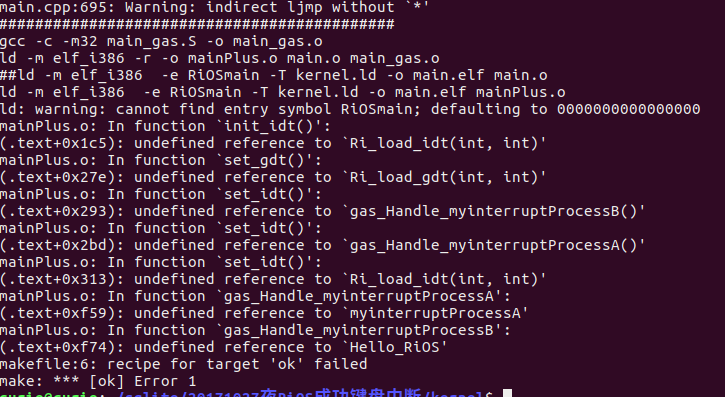
\includegraphics[width=14cm]{pic/assets/problems/problem01_1}
        \caption{问题01-1}	\label{problem01_1}	\end{figure}


一直找不到原因,我将编译后的机器码反汇编成.asm文件找原因,如图~\ref{problem01_2}~所示.	

\begin{figure}[!htbp]
		\centering	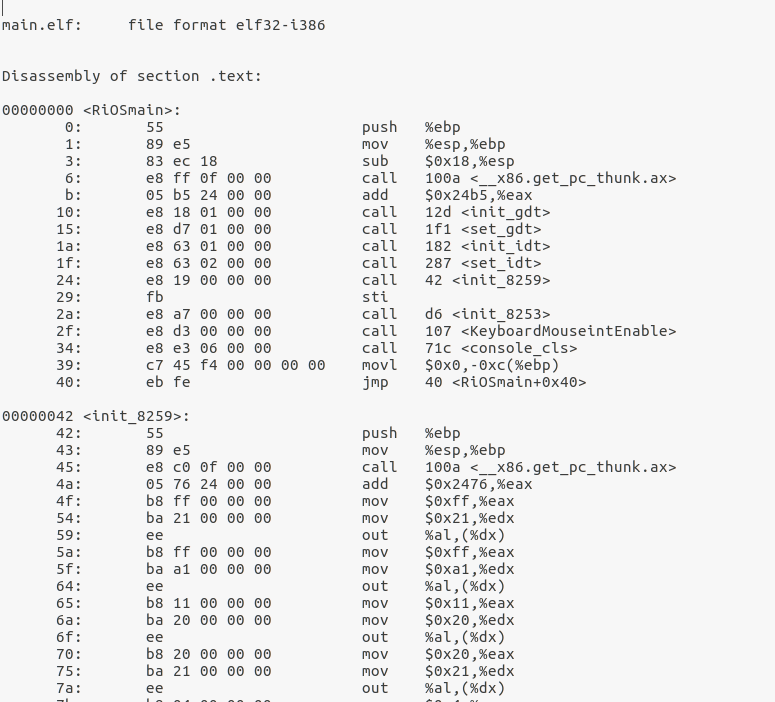
\includegraphics[width=14cm]{pic/assets/problems/problem01_2}
        \caption{编译.c文件时的结果}	\label{problem01_2}	\end{figure}
        
Linux命令:objdump -S -D main.elf >main.asm
              
之前编译正常.c文件时的编译结果如图~\ref{problem01_2}~所示.	


可以看到,我的函数名RiOSmain和init\_8259在编译之后是保留原来的字的。

Linux命令:

g++  -nostdinc -I.  -fpermissive -fno-stack-protector -c main.cpp -m32 -o main.o

objdump -S main.o >main.asm


\begin{figure}[!htbp]
    \centering	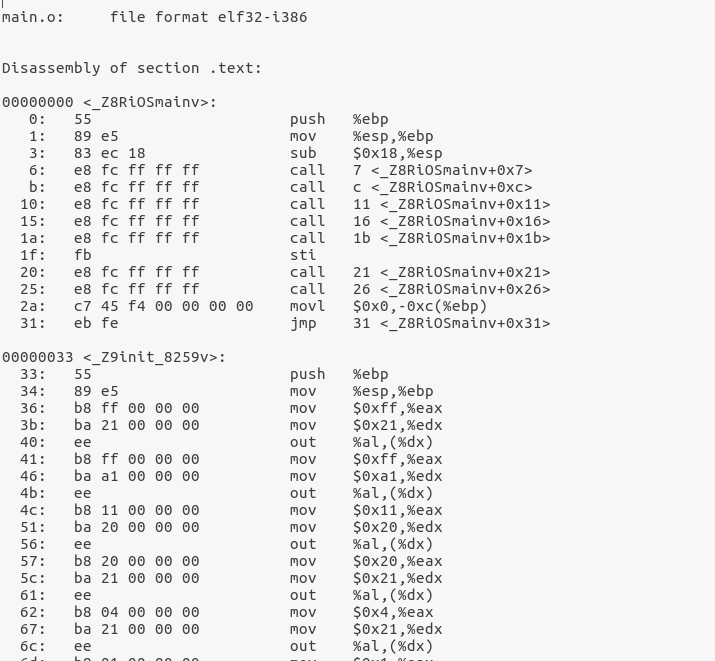
\includegraphics[width=14cm]{pic/assets/problems/problem01_3}
    \caption{编译同样内容的.cpp文件时的结果}	\label{problem01_3}	\end{figure}

此时我惊讶地发现,在gcc或g++对.cpp文件编译时,原来RiOSmain的函数名变成了Z数字RiOSmainv,
即gcc是这样处理的函数到标号的映射是标号:Z数字函数名v,加上了前缀后缀,这样根据名字去链接必然失败.

解决方法是将C++源程序保存为.cc文件,在头文件的把函数声明包在extern "c"{}之中,
这样C++的函数编译后就能和C编译后的函数兼容.
        
\subsection{问题解决后的结果样式}

\begin{minted}{c}
    /*this is hello.h*/
    #ifdef __cplusplus
    extern "C" {
    #endif /* __cplusplus */
    void hello_cplusplus();
    #ifdef __cplusplus
    }
    #endif /* __cplusplus */    
\end{minted}
extern "C"的意思,是让C++编译器(不是C编译器,而且是编译阶段,不是链接阶段)
在编译C++代码时,为被extern “C”所修饰的函数在符号表中按C语言方式产生符号名
(比如前面的add),而不是按C++那样的增加了参数类型和数目信息的名称(\_Z3addii)。

展开来细说,就是:如果是C调用C++函数,在C++一侧对函数声明加了extern "C"后
符号表内就是add这样的名称,C程序就能正常找到add来调用;如果是C++调用C函数,
在C++一侧在声明这个外部函数时,加上extern "C"后,C++产生的obj文件符号表内就
也是标记为它需要一个名为add的外部函数,这样配合C库,就一切都好。

特地写了一个简单的程序来验证一下,加深印象,如图~\ref{problem02_1}~所示.	

\begin{figure}[!htbp]
		\centering	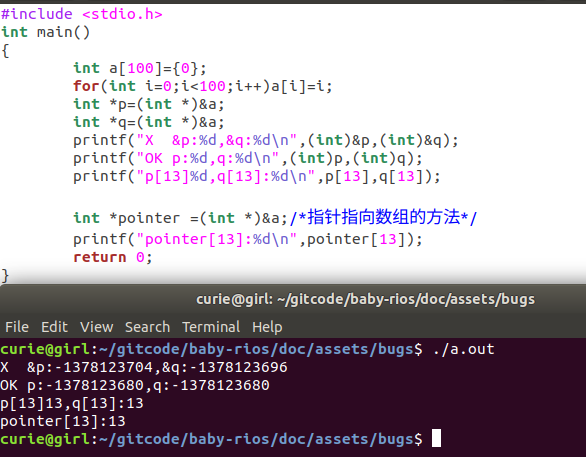
\includegraphics[width=14cm]{pic/assets/problems/problem02_1}
        \caption{问题02-1}	\label{problem02_1}	\end{figure}
        
\begin{minted}{c}
    #include <stdio.h>
    int main()
    {
        int a[100]={0};
        for(int i=0;i<100;i++)a[i]=i;
        int *p=(int *)&a;
        int *q=(int *)&a;
        printf("X  &p:%d,&q:%d\n",(int)&p,(int)&q);
        printf("OK p:%d,q:%d\n",(int)p,(int)q);
        printf("p[13]%d,q[13]:%d\n",p[13],q[13]);
    
        int *pointer =(int *)&a;/*指针指向数组的方法*/
        printf("pointer[13]:%d\n",pointer[13]);
        return 0;
    }
\end{minted}

\section{问题02:指针使用}
\subsection{问题描述}
指针使用错误.
\subsection{问题具体样式}
代码见下.

联合体相当于是个实体,而数组int a[10]中的a就是个指针,若在指针前面,
再加上取地址符\mintinline{c}!&!就成了指针的地址,在联合体前面加取地址符就是指向联合体的指针.
我之前错误地在指针前面加了取地址符,导致间接寻址都无效.

\subsection{问题分析及解决方案}
\begin{minted}{c}
    /*这里是修改好后的正确写法*/
    u8 two_sectors[1024]={0};
    IDE_read_sector((void *)two_sectors, DATA_BLK_NR_TO_SECTOR_NR(p_ft->f_inode->i_zone[7]));
    /*之前这里错误地写成了,IDE_read_sector((void *)&two_sectors,多了个&造成大错*/
    union free_space_grouping_head g_head;
    u8 * p1 = (u8 *)&g_head ;IDE_write_sector((void *)p1,sector_num );
\end{minted}

\subsection{问题解决后的结果样式}
正常编译运行.

\section{问题03:中断的EOI信号}
\subsection{问题描述}
中断只能执行一次.

\subsection{问题具体样式}
比如键盘中断,按下一个键,可以在屏幕上显示相应字符,
但是再按键盘一点也没有反应.
如图~\ref{problem03_1}~所示.	

\begin{figure}[!htbp]
		\centering	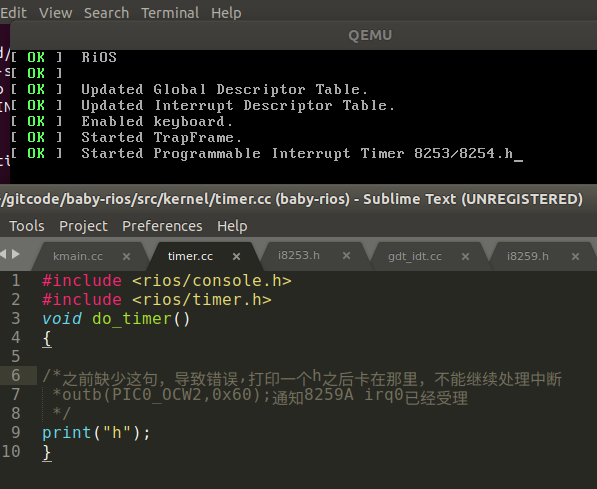
\includegraphics[width=14cm]{pic/assets/problems/problem03_1}
        \caption{问题03-1}	\label{problem03_1}	\end{figure}

\subsection{问题分析及解决方案}
在中断处理函数中通过in out指令告知8259A中断已经被处理,不然将会一直卡死在那里,不会受理下一次中断.

解决方案:方法一是给8259A发EOI信号,即为\mintinline{c}!outb(PIC0_OCW2,0x60)!,即outb(0x20,0x60);
方法二是采用自动EOI方式,目前RiOS采用后者,一下这两句分别给主片和从片设为自动EOI模式.

\begin{minted}{c}
outb_wait(0x20 + 1, 0x3); // Auto EOI in 8086/88 mode
outb_wait(0xa0 + 1, 0x3); // Auto EOI in 8086/88 mode
\end{minted}

\subsection{问题解决后的结果样式}
正常响应中断,不会按下一个键就卡住了.

\section{问题04:triple fault}
\subsection{问题描述}
这个问题可能是'triple fault'.

\subsection{问题具体样式}
早期写内核时遇到一个bug,用grub引导过去之后一按键盘就重启,一按找不到原因. 

\subsection{问题分析及解决方案}
初步猜测两个原因 一是在gdt没有正确设置的情况下去写中断处理的代码,
二可能是没有把所有陷阱门搞个处理函数.

在网上找到大致符合我症状的描述(http://www.osdever.net/bkerndev/Docs/gdt.htm).

Note that GRUB already installs a GDT for you, 
but if we overwrite the area of memory that GRUB was loaded to, 
we will trash the GDT and this will cause what is called a 'triple fault'.
 In short, it'll reset the machine. What we should do to prevent that 
 problem is to set up our own GDT in a place in memory that we know 
 and can access. This involves building our own GDT, telling the
  processor where it is, and finally loading the processor's CS, DS, 
  ES, FS, and GS registers with our new entries. The CS register
   is also known as the Code Segment. The Code Segment tells the 
   processor which offset into the GDT that it will find the
    access privileges in which to execute the current code. 
    The DS register is the same idea, but it's not for code, 
    it's the Data segment and defines the access privileges for
     the current data. ES, FS, and GS are simply alternate DS 
     registers, and are not important to us.

我们利用GRUB进入保护模式,这里GRUB应该给我们默认设置了GDT,但是如果我们把gdt的地方覆盖了,
将会引发异常,具体叫做'triple fault',这或许就是原因.

想到这里,我觉得在设置IDT之前,我们应当自己先把GDT设置好,GRUB默认设的可能会覆盖,因此这是有必要的.
\subsection{问题解决后的结果样式}
当我先设置GDT再设置IDT之后,不再出现一按键盘就重启的现象,一切正常了.



\section{问题05:打开的文件不对应}
\subsection{问题描述}.
open函数不能正确打开文件.
\subsection{问题具体样式}
通过open返回的fd对应了其他文件,错乱了.如图~\ref{problem05_1}~所示.本来要显示的是
大文件《简爱》(jane.txt),然而打印出来的是hamlet.txt这么一个小段的话.	

\begin{figure}[!htbp]
		\centering	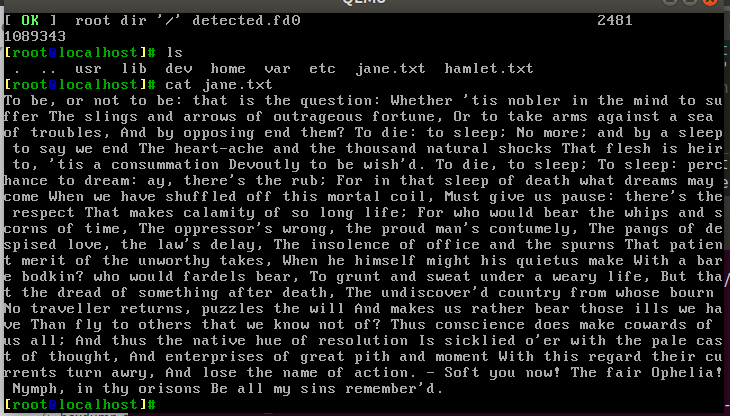
\includegraphics[width=14cm]{pic/assets/problems/problem05_1}
        \caption{问题05-1}	\label{problem05_1}	\end{figure}

\subsection{问题分析及解决方案}
文件系统中,我们有三个表,这三个表联系紧密,他们之间的关系类似于索引,使用时要确保这种索引关系要时刻保持,
不然这个链就断了,之前没有\mintinline{c}!current->filp[fd]->f_inode!指向活动inode表,导致虽然已经正确写入磁盘,
活动inode表里也有,但是 甲=>乙=>丙 两个指针中有一个没有指向正确的地方,这就导致最终指不到正确的inode,
造成错误.

错误原因在于在open 函数中我在最后漏写了这一句:
    
\mintinline{c}!current->filp[fd]->f_inode = &active_inode_table.inode_table[active_inode_table_nr];!

\subsection{问题解决后的结果样式}
正常.

下面几个问题都比较小,比较容易解决,有些就合起来描述了.

\section{问题06:同步性}

\subsection{问题描述}
close 函数也存在和bug09中open函数类似的问题,那就是没有保持那三个表的同步性.
\subsection{问题分析及解决方案}
\begin{minted}{c}
    /*更正时,在close新添加的语句*/
    for(j=0;j<MAX_ACTIVE_INODE;j++)
    		if(active_inode_table.inode_table[j].i_ino==filp->f_inode->i_ino)
    			break;
    	memset(&active_inode_table.inode_table[j],0x00,sizeof(m_inode));
\end{minted}
这样在close时也把活动inode清理,这就不会出差错了.

\section{问题07:编译选项}
\subsection{问题描述}
编译报错.如图~\ref{problem07_1}~所示.	

\begin{figure}[!htbp]
		\centering	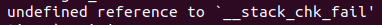
\includegraphics[width=14cm]{pic/assets/problems/problem07_1}
        \caption{问题07-1}	\label{problem07_1}	\end{figure}

\subsection{问题具体样式}
undefined reference to `\_\_stack\_chk\_fail'
\subsection{问题分析及解决方案}
解决方法:在编译时,在CFLAGS后面加上-fno-stack-protector

-fno-stack-protector 

\subsection{问题解决后的结果样式}
正常编译.

\section{问题08:键盘支持}
\subsection{问题描述}
在qemu虚拟机中没问题,按一个键打印一个字符,但到了实体机按一次打印两个相同字符

\subsection{问题具体样式}
原理:按一个键打印两个字符,因为一次是Make code,一次是Break Code.
键盘的扫描码Scan Code,通码Make code,断码Break Code 用户按键盘上的字母,
硬件底层会产生对应的Scan Code,而且是按下那一刻产生一个通码Make code,
释放的时候产生一个断码Break code。即你从按下一个键盘上的字母,
到手松开,实际上对应着一个通码Make Code和一个断码Break Code,
两者概念上都属于扫描码Scan Code。

\subsection{问题分析及解决方案}
解决方法:判断键盘状态
\subsection{问题解决后的结果样式}
正常.

\section{问题09:对大文件的支持}
\subsection{问题描述}
支持不了大文件
\subsection{问题具体样式}
大一点的文件只能找到它的前面小部分,后面就找不到、显示不出来了.
\subsection{问题分析及解决方案}
i\_size当时设的值太小了,当时没有考虑到后来文件变得很大的时候.

当时开始设的文件大小i\_size类型是u8,也就是8位二进制数,但可以看到我的jane.txt内容相当多,
是简爱一本书的内容,大小有1089343,用十六进制表示是0x109f3f,明显8位二进制数早已不能表示它,
发生溢出.当我的文件大小没有超过8位时,cat jane.txt和cat hamlet.txt都能正常工作,但是此时文件大小比较大,
i\_size这一项错误了,导致显示jane.txt时错误地显示了hamlet.txt的内容.故需要修改i\_size类型,
使其为32位,同时,我的inode大小是固定好的,还要调整其他项,使inode大小不发生改变.

这只是其中原因之一,之二是我还没有支持二级间地址访问,所以一个文件最大容量受限,容纳几kB还行,
但尚不能容纳几MB大小的单个文件.

\subsection{问题解决后的结果样式}
完善代码后支持了大文件.

\section{问题10:少括号}

这是个非常简单的错误,但找起来却不轻松我本要一个数除以(80*25),结果错误地写成int times = len/80 * 25;
这样实际上变成了(len/80)25,导致错误.应该写成int times = len/(8025);



% \clearpage